\section{CanJS}
\label{ch:canjs}

\subsection{Présentation}

Le framework CanJS est issu du framework Javascript MVC. Il s'agit en fait de l'extraction du noyau et il est décomposé en modules pour coller exactement aux besoins de l’application sans embarquer des Kilos octects de fonctionnalités inutiles. La nouvelle version de Javascript MVC se basera sur CanJS pour assurer l’inter-compatibilité des deux frameworks.

Le grand intérêt de CanJS est de fournir des objets « Model » pour stocker nos données, y associer des fonctions de mise à jour coté serveur personnalisables et des événements auxquels attacher des actions. Mieux, il gère automatiquement, grâce à son système de templates, la mise à jour de toutes les vues associées à un modèle lorsque ce dernier est modifié.

CanJS est composé de:
\begin{itemize}

    \item[\textbullet]
	can.Construct - hérite des fonctions du constructeur
	
	\item[\textbullet]
	can.Observe - clé valeur contraignante

	\item[\textbullet]
    can.Model -  permet de connecter une interface JSON-REST
	
	\item[\textbullet]
    can.View - chargement du modèle, mise en cache

	\item[\textbullet]
    can.EJS - modèles contraignant direct

	\item[\textbullet]
    can.Control - liaisons d’évnements déclaratif
    
	\item[\textbullet]    
    can.Route - support du bouton précédent et des onglets
    	
\end{itemize}

Il prend également en charge un riche ensemble d’extensions et plugins.

\subsection{Caractéristiques vs Poids}


En plus de jQuery, CanJS fait 8.5kb. A titre d’exemple voici quelques autres bibliothèques MVC (compressé avec gzip):

\begin{itemize}

	\item[\textbullet]
	8.97kb pour Backbone (avec Underscore.js)

	\item[\textbullet]
    24kb pour AngularJS

	\item[\textbullet] 
    13kb pour Knockout

	\item[\textbullet] 
    37kb pour Ember
    
    \item[\textbullet] 
    15kb pour Batman

\end{itemize}

Pour être juste, le poids est trompeur, car chaque bibliothèque possède un ensemble différent de fonctionnalités. Cependant, CanJS fournit tout ce dont vous avec besoin pour créer une applications coté client riche, avec la bibliothèque la plus légère parmi celle comparé.
Par comparaison Backbone.js est livré le micro template Underscore.js, mais ceux-ci ne se compare pas à la puissance de EJS. La plupart des applications réseau de base comprennent également un moteur de templates qui ajoute du poids à la bibliothèque. 

\subsection{Facilité d’utilisation}

CanJS bénéficie d’une courbe d’apprentissage plus facile que n’importe quelles autres biblothèques. CanJS bénéficie d’une bonne documentation. Il permet de se faire la main avec la page de présentation, puis de plonger plus profondément en lisant chaque méthodes et classe dans la page de documentation. CanJS permet de voir comment les applications sont construites en parcourant les exemples, en lisant les annotations et en regardant les jeux de tests. Un blog permet d’en savoir toujours plus sur CanJS, et il est possible de poser des questions sur le forum. Twitter ou d’obtenir un support premium, de formations ou de conseil.

\subsection{Prévention des fuites mémoire}

CanJS empêche les fuites de mémoire qu’un développeur ne connait problablement pas et a dans son application. Les applications JavaScript ont communément des fuites mémoire de deux sources: les gestionnaires d’évenements et les objets inutilisées.
Autant dire qu’il s’agit d’un problème critique pour les client MVC. CanJS gère ces fuites automatiquement ce qui rend presque impossible une fuite mémoire dans l’application.

\subsection{Performance}

CanJS est optimisé pour la performance dans des domaines clés.
Par exemple la liaison en temps réel est optimisé pour les performances en modifiant directement et exactement ce qui doit être mis à jour, plutôt que le modèle en entier.

Voici un schéma mesurant les performance de CanJS en fonction d’autres frameworks.


\begin{center}
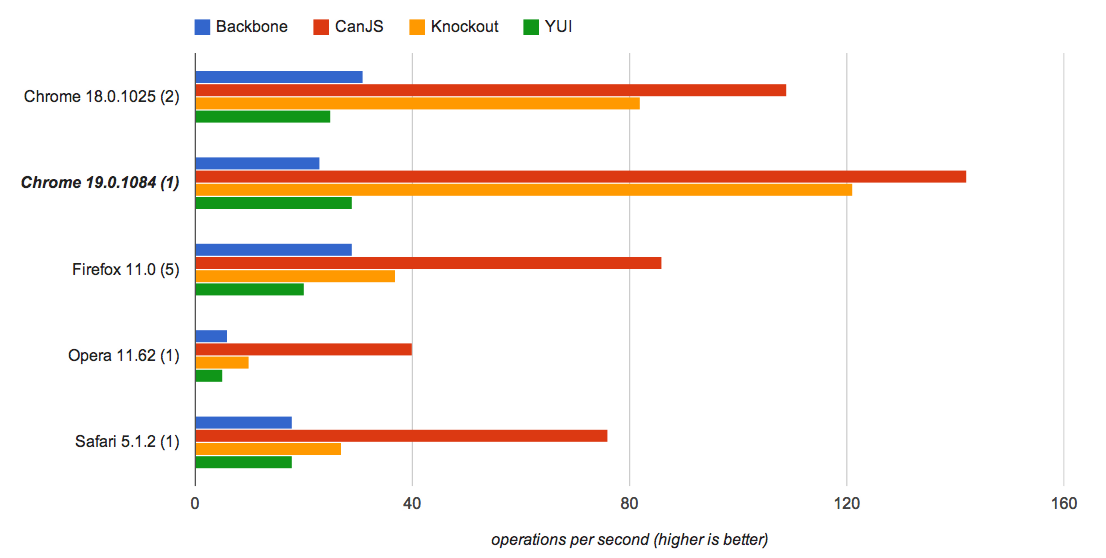
\includegraphics[scale=0.4]{img/performance_livebind.png}
\label{Graphique performance CanJS}
\end{center}

\subsection{Support de librairie}

CanJS permet d'intègrer cinq des bibliothèques les plus couramment utilisés pour l’accès au DOM:

\begin{center}

\includegraphics[scale=0.5]{img/CanJSlibraries.png}
\label{Graphique bibliothèque CanJS}
\end{center}

Cela donne la possibilité de choisir la bibliothèque préférée ou passer même facilement par une autre bibliothèque sans avoir a réécrire la couche MVC de votre application.

Il y’a une intégration profonde avec chaque bibliothèque afin de permettre une utilisation complète peut importe la librairie choisie.